% !TEX root =  ../main_manuscript.tex 

\section{Introduction}
\label{sec:introduction}
Prostate cancer is the second most frequently diagnosed cancer in men worldwide \cite{GlobalCancerStats2012}. However, many of the diagnosed tumors are clinically insignificant (over-diagnosed) \cite{etzioni2002overdiagnosis}. To avoid further over-treatment, patients diagnosed with low-grade prostate cancer are commonly advised to join active surveillance (AS) programs. In AS, serious treatments such as surgery, chemotherapy, or radiotherapy are delayed until cancer progresses. Cancer progression is routinely examined via serum prostate-specific antigen (PSA) levels: a protein biomarker, digital rectal examination (DRE) score: a measure of the size and location of the tumor, medical imaging, and biopsies etc.

While larger values for PSA and/or larger score for DRE, may indicate cancer progression, biopsies are the most reliable cancer progression examination technique used in AS. When a patient's biopsy Gleason grading becomes larger than 6 (positive biopsy), AS is stopped and the patient is advised treatment for cancer progression \cite{bokhorst2015compliance}. However, biopsies are invasive, painful, and prone to medical complications \cite{ehdaie2014impact,fujita2009serial}. Hence, they are conducted intermittently until a positive biopsy. Consequently, at the time of a positive biopsy, cancer progression is observed with a delay of an unknown duration. This delay is defined as the difference between the time of the positive biopsy and the unobserved true time of cancer progression. Thus, the decision of conducting a biopsy requires a fine compromise between the burden of a biopsy, and the potential duration of the delay in the detection of cancer progression.

In AS, a delay in detection of cancer progression around twelve to fourteen months is assumed to be unlikely to substantially increase risk for adverse downstream outcomes \cite{inoue2018comparative,carvalho}. However, for biopsies there is little consensus on the time gap between them \cite{loeb2014heterogeneity}. Majority of the AS programs focus on minimizing only the delay in detection of cancer progression, by scheduling biopsies annually (most frequent schedule) for all patients. A drawback of annual biopsies, and other fixed/heuristic schedules\cite{inoue2018comparative}, is that they ignore the large variation in the time of cancer progression of AS patients. While they may work well for patients who progress early (\textit{fast progressing}) after inclusion in AS, but for a large proportion of patients who do not progress until late (\textit{slow progressing}) in AS (see Figure \ref{fig:npmle_plot}), many unnecessary burdensome biopsies are scheduled. To mediate the burden between the fast and slow progressing patients, the world's largest AS program, Prostate Cancer Research International Active Surveillance (PRIAS) \cite{bokhorst2016decade}, schedules annual biopsies only for patients with a small PSA doubling time\cite{bokhorst2015compliance}. For everyone else, PRIAS schedules biopsies at following fixed follow-up times: year one, four, seven, and ten, and every five years thereafter. Despite this effort in PRIAS, a patient may get scheduled for four to ten biopsies over a period of ten years. Consequently, patients may not always comply with the biopsy schedule \cite{bokhorst2015compliance}. This can lead to the original problem of delayed detection of cancer progression, and reduce the effectiveness of AS.

\begin{figure}[!htb]
\captionsetup{justification=justified}
\centerline{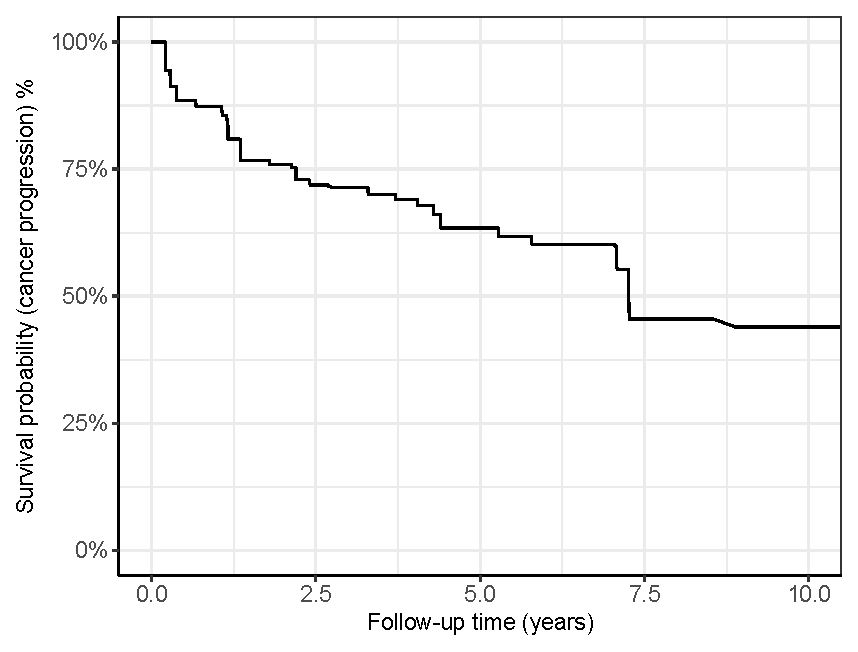
\includegraphics[width=\columnwidth]{images/npmle_plot.eps}}
\caption{\textbf{Estimated survival probability of cancer progression in AS}: for patients in the Prostate Cancer Research International Active Surveillance (PRIAS) dataset. Nearly 50\% patients (\textit{slow progressing}) do not progress in the ten year follow-up period. Estimation is done using a nonparametric maximum likelihood estimate, of the distribution function for interval censored cancer progression times observed in PRIAS \citep{turnbull1976empirical}.}
\label{fig:npmle_plot}
\end{figure}

%Three reasons for why median and not mean:
%1. mean has decimals, hard to interpret
%2. median and IQR are useful coz distributions are skewed
%3. median also corresponds to 50% of those patients who never progress. Thus X axis is also having the interpretation: Burden for patients who never progess. and Y axis: median beenfit for patients who progress at the burden of those who never progress.
%4. no point showing mean for this plot and showing median (IQR) everywhere else
\begin{figure}[!htb]
\captionsetup{justification=justified}
\centerline{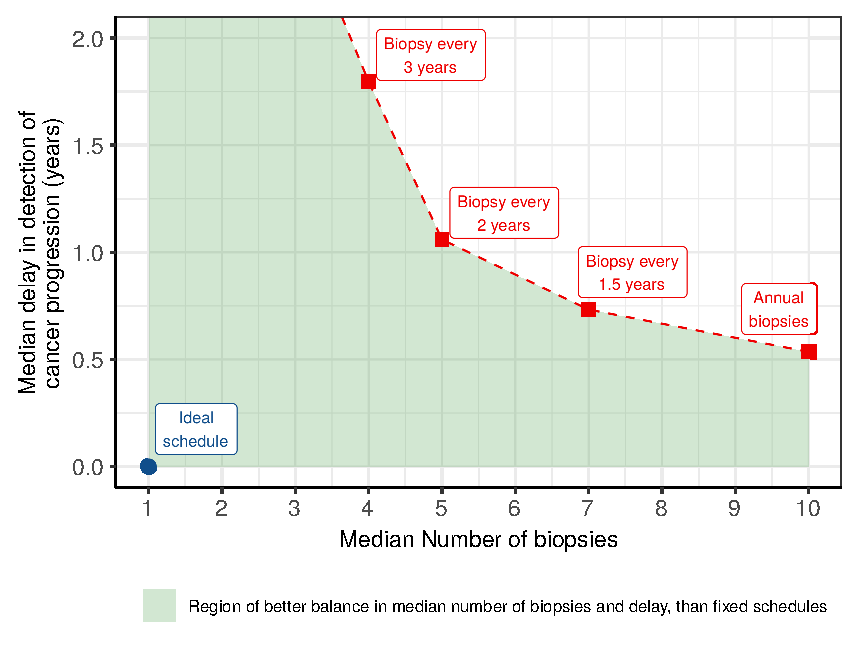
\includegraphics[width=\columnwidth]{images/better_balance_intro.eps}}
\caption{\textbf{Burden-benefit frontier}: Estimated median number of biopsies (more are burdensome), and median delay in detection of cancer progression (less is beneficial), due to various currently practiced fixed/heuristic biopsy schedules (red squares), over a follow-up of ten years. Estimation is based on cancer progression times generated using the survival probability curve in Figure~\ref{fig:npmle_plot}. Using personalized decision making for biopsies, we intend to better balance the number of biopsies and the delay (green region), than currently practiced schedules. An ideal biopsy schedule (blue circle) will schedule only one biopsy, exactly at the true time of cancer progression.}
\label{fig:better_balance_intro}
\end{figure}

This article is motivated by the need to better balance the number of biopsies (more are burdensome), and the delay in detection of cancer progression (less is beneficial), than practiced currently (see Figure~\ref{fig:better_balance_intro}). We intend to achieve this by personalizing the decision of conducting biopsies at follow-up visits. To this end, we utilize the data of the patients of the PRIAS study. Personalized decision making has received much interest in the literature, especially for the screening of various cancers, by exploiting Markov decision process models \cite{ayer2012or, akhavan2017markov,erenay2014optimizing}. Similar models have also been used for personalizing the pre-diagnosis prostate cancer screening strategy\cite{zhang2012optimization,krahn1994screening}. However, in post-diagnosis AS programs, to the best of our knowledge, only fixed/heuristic approaches \cite{inoue2018comparative,carvalho}, or PSA doubling time \cite{bokhorst2015compliance} have been employed for deciding the time of biopsies.

\begin{figure}[!htb]
\captionsetup{justification=justified}
\centerline{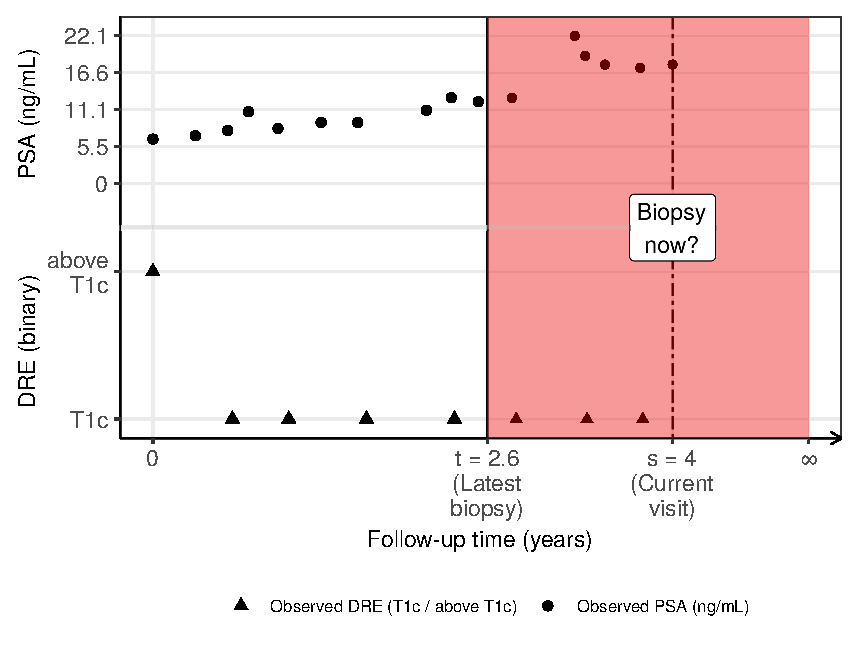
\includegraphics[width=\columnwidth]{images/obsDataPlot_2340.eps}}
\caption{\textbf{The personalized decision making problem}: Available data of a patient $j$, who had his latest negative biopsy at $t=2.6$ years. The shaded region shows the time period in which the patient is at risk of cancer progression. His current pre-scheduled follow-up visit for measurement of DRE and PSA is at $s=4$ years. Using his entire history of DRE $\mathcal{Y}_{dj}(s)$ and PSA $\mathcal{Y}_{pj}(s)$ measurements up to the current visit $s$, and the time of the latest biopsy $t$, we intend to make a decision on scheduling a biopsy at the current visit.}
\label{fig:obsDataPlot_2340}
\end{figure}

In this work, we make a patient-specific decision of biopsy at a patient's pre-scheduled follow-up visit (logistical considerations) for DRE and PSA measurements. In comparison to the work referenced above, we make this decision using the entire history of DRE scores, PSA levels and the estimated rate of change of PSA (PSA velocity), and results of the latest biopsy of a patient up to the latest follow-up visit. We achieve this by utilizing joint models for time-to-event and longitudinal data \cite{tsiatis2004joint,rizopoulos2012joint}. Joint models consist of a longitudinal mixed effects sub-model for periodically measured outcomes such as DRE and PSA, and a relative risk sub-model for modeling the time of cancer progression. The association between these three outcomes, and especially the fact that the DRE and PSA measurements are missing after the detection of cancer progression, is modeled using patient-specific random-effects \cite{laird1982random}. By estimating the parameters of the model jointly, we first obtain a full specification of the joint distribution of the time of cancer progression, and DRE and PSA measurements. We then use it at a patient's follow-up visit, to estimate the patient-specific cumulative risk of observing cancer progression at that visit. If that risk is higher than a certain threshold, our method proposes a biopsy at the same follow-up visit. We exploit fixed risk thresholds used in standard clinical settings, as well as we propose a methodology to choose risk thresholds on the basis of their classification accuracy.

We evaluate the personalized risk based biopsy approach, and the currently practiced fixed/heuristic, PRIAS biopsy schedules on the basis of their utility for the patients. That is, the number of biopsies they schedule, and the corresponding delay incurred in the detection of cancer progression. To compare the aforementioned schedules on these criteria, we conduct an extensive simulation study. For a realistic comparison, we simulate a replica of the population of the PRIAS patients, using the joint model fitted to the PRIAS dataset.

The rest of the article is structured as follows: The details of the joint modeling framework and biopsy decision making methodology are presented in the \hyperref[sec:methods]{Methods} section. The details of the simulation study and the corresponding results are presented in \hyperref[sec:methods]{Methods} and \hyperref[sec:results]{Results} sections, respectively.